
% JuliaCon proceedings template
\documentclass{juliacon}
\setcounter{page}{1}

\usepackage{amsmath}

\begin{document}

% **************GENERATED FILE, DO NOT EDIT**************

\title{DMRGenie: Graphical interface for entanglement renormalization}

\author[1]{Kiana Gallagher}
\author[1]{Aaron Dayton}
\author[2]{Drew Leske}
\author[2]{Sarah Huber}
\author[134]{Thomas E. Baker}
\affil[1]{Department of Physics \& Astronomy, University of Victoria, Victoria, British Columbia V8P 5C2, Canada}
\affil[2]{Research Computing Services, University of Victoria, Victoria, British Columbia V8P 5C2, Canada}
\affil[3]{Department of Chemistry, University of Victoria, Victoria, British Columbia V8P 5C2, Canada}
\affil[4]{Centre for Advanced Materials and Related Technologies, University of Victoria, Victoria, British Columbia V8P 5C2, Canada}

\keywords{Julia, Genie, DMRjulia, TENPACK, Entanglement Renormalization, Tensor Networks, Graphical User Interface}

\hypersetup{
pdftitle = {DMRGenie: Graphical interface for entanglement renormalization},
pdfsubject = {JuliaCon 2022 Proceedings},
pdfauthor = {Kiana Gallagher, Aaron Dayton, Drew Leske, Sarah Huber, Thomas E. Baker},
pdfkeywords = {Julia, Genie, DMRjulia, TENPACK, Entanglement Renormalization, Tensor Networks, Graphical User Interface},
}



\maketitle

\begin{abstract}

We discuss implementation of a graphical user interface for tensor operations in scientific simulations related to entanglement renormalization. This software, which we call DMRGenie, based on its heavy reliance on Genie which is a well-known software package for web applications. We also discuss the deployment of the software. Scientific simulations with tensor network-based framework of quantum algorithm methods is now possible through this tool without length start-up or learning times.

\end{abstract}


\section{Introduction}

On one hand, for ideas to be implemented computationally, a need arises for easy-to-use high level languages. "On the other hand, scientific programming often requires computational resources at scale, driving optimization and performance requirements. To accomplish this second demand, a low-level language is required to control as much as possible in an implementation of an algorithm. This split between needs for different programming projects is known as the two-language problem.

The Julia programming language is a good if not great attempt to solve this two-language problem. By optimizing for loops, programs can be created in a rapid manner but still achieve performance on par with lower-level languages such as C++. 

In any scientific endeavour, the need to use numerical techniques is highly necessary. And for new advances to be made, new methods must be able to be implemented into any given language to evolve beyond the state-of-the-art. For anyone developing new algorithms, the need for a programming framework that enables as many solutions of the two-language problem as possible is necessary, making a Julia a strong contender for algorithmic development.

%For any algorithm development team, the need for custom software that displays as many solutions of the two-language problem is necessary, making Julia a strong option for use in algorithm development.

Quantum information methods have become a tantalizing path to creating new algorithms and methods. These range from quantum algorithms implemented on quantum computers \cite{nielsen2010quantum} (but since no perfect quantum computer exist, simulations with classical methods are still required) to entanglement renormalization techniques.\footnote{This class of methods is more commonly referred to as tensor networks, simply, but with the rise of machine-learning and other methods particularly in quantum chemistry that are formulated on tensor networks, a distinguishing name is required. We choose to expand the usage of the term from Ref.~\cite{vidal2007entanglement} since all methods are fundamentally optimizing over quantities relevant for quantum information ({\it i.e.}, the entanglement) and renormalization was originally introduced to describe this class of methods \cite{wilson1983renormalization,krishna1980renormalization}. The methods required to implement an algorithm in this context is different from other contexts, notably machine learning.} 

\begin{figure}
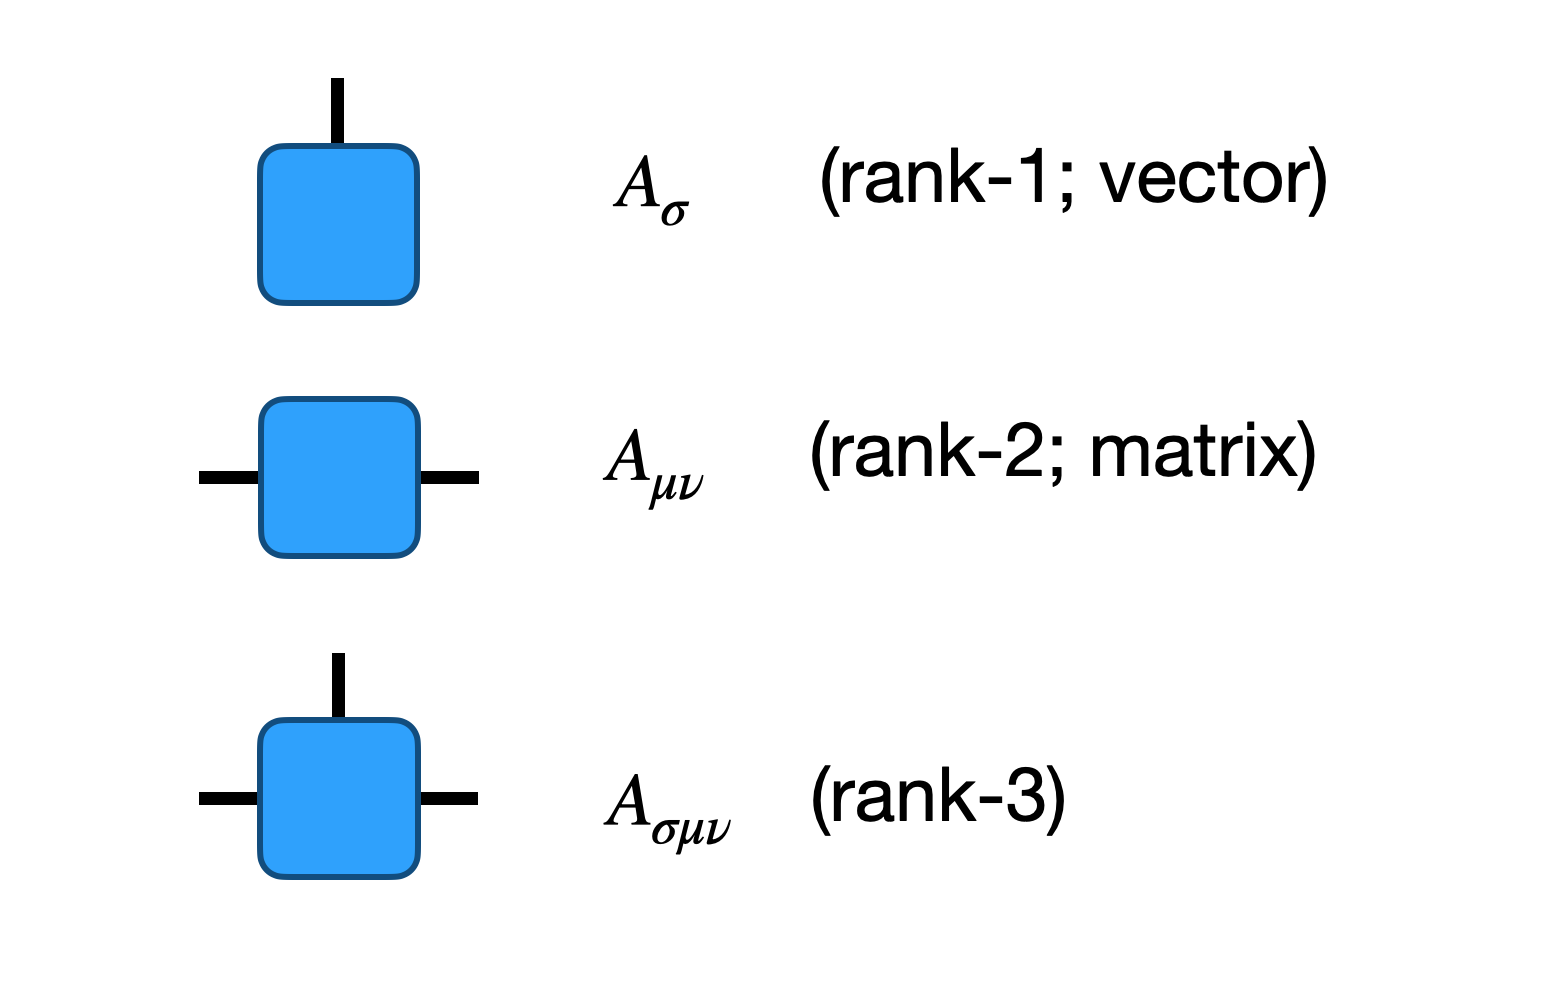
\includegraphics[width=\columnwidth]{diagram.png}
\caption{Shown are diagrams for rank-1, 2, and 3 tensors. Each line signifies another index on the tensor.
\label{diagram}
}
\end{figure}

Methods of entanglement renormalization use quantities native to quantum information ({\it i.e.}, the density matrix or the entropy) in order to optimize a a quantum problem to find solutions to the eigenvalue problem (Schr\"odinger's equation) \cite{townsend2000modern}. Entanglement renormalization techniques are formulated on a graph of tensors and have definite rules for tensor operations. Because tensor computations and operations can be cumbersome to represent mathematically in index notation, the field has adopted a diagram notation that allows for the improved communication of algorithms. Namely, the rank of the tensor corresponds to the number of lines on the diagram \cite{penrose1971angular}. An example is shown for rank-1, 2, and 3 tensors in Fig.~\ref{diagram}. 

Realistically, only about a rank-14 tensor can be represented on a laptop machine. This is because each of the tensor indices has dimension of at least two, approaching the memory limitations of these devices. Therefore, the rank of the tensors represented here are small and often only a few indices are present.

When contracting two tensors together, one can connect two indices on the same tensor ({\it i.e.}, tracing over indices) or between tensors (contraction). When representing a network of tensors, the indices are typically not kept track of. Instead, indices that point towards each other or have matching labels are assumed to be contracted eventually. This rarely causes confusion when implementing algorithms.

\begin{figure}
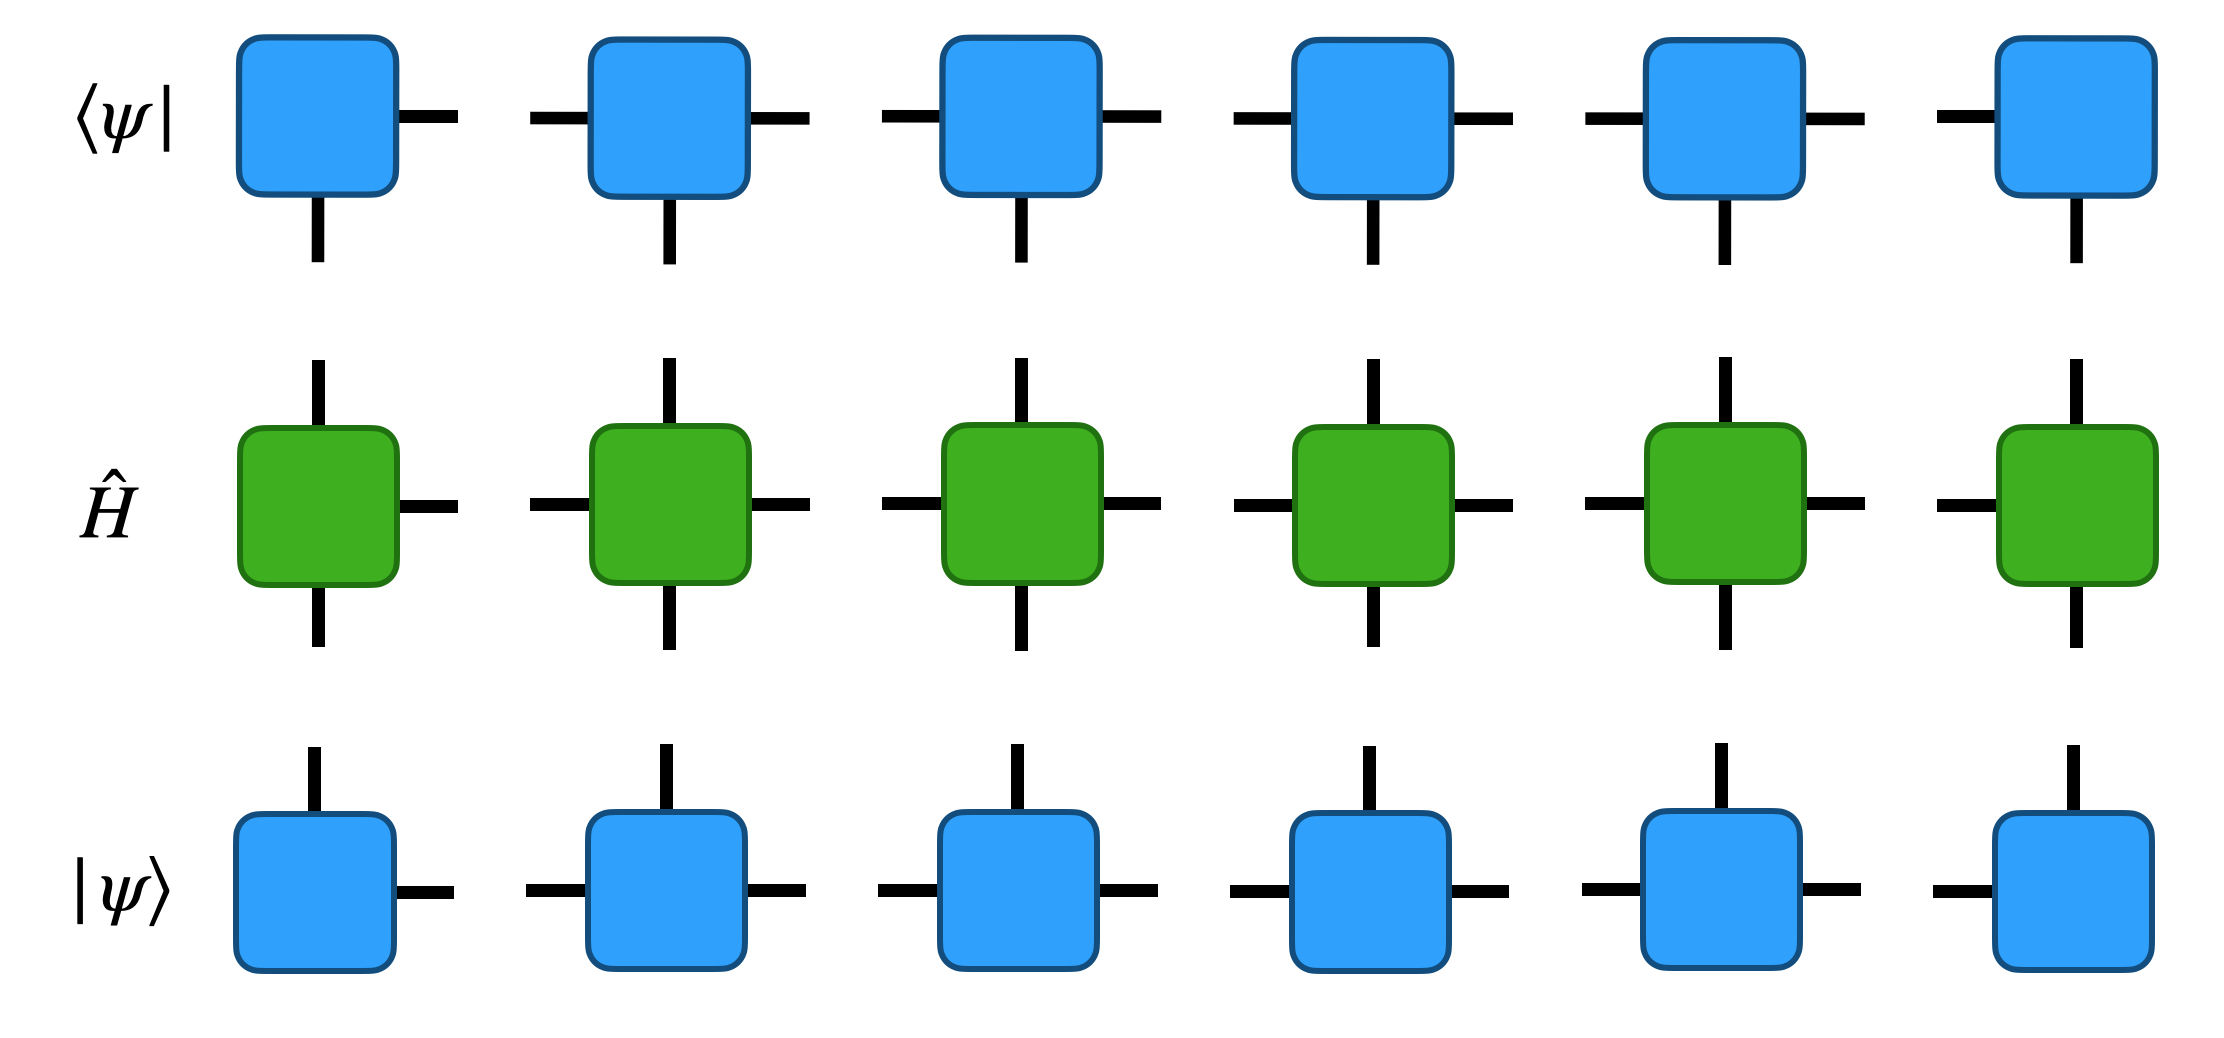
\includegraphics[width=\columnwidth]{network.png}
\caption{The expectation value of an operator $\hat H$ is shown in tensor diagram notation for a 6-site system. When contracted, this would give $\langle\hat H\rangle$, or the energy $E$ if $\hat H$ is the Hamiltonian. The wavefunction on the bottom row alone would be represented as in the text (Eq.~\ref{mpsform}), which is far more intricate.
\label{network}
}
\end{figure}

The use of the diagram notation is useful for representing large numbers of tensors in a coherent way without representing cumbersome mathematics (see Fig.~\ref{network}). For example, the wavefunction when decomposed through a series of reshapes and singular value decompositions (SVD) takes the form \cite{bakerCJP21}
\begin{align}\nonumber
|\psi\rangle&=\sum_{\substack{\sigma_1\sigma_2\sigma_3\\\sigma_4\sigma_5\sigma_6}}\sum_{\substack{a_1a_2a_3\\a_4a_5}}A^{\sigma_1}_{a_1}A^{\sigma_2}_{a_1a_2}A^{\sigma_3}_{a_2a_3}A^{\sigma_4}_{a_3a_4}A^{\sigma_5}_{a_4a_5}A^{\sigma_6}_{a_5}\\
&\quad\quad\quad\quad\quad\quad\quad\quad\times|\sigma_1\sigma_2\sigma_3\sigma_4\sigma_5\sigma_6\rangle
\label{mpsform}
\end{align}
which is far more intricate than the diagram notation but conveys no extra information. Any quantum operator (for example, the Hamiltonian) can be decomposed into a similar site-by-site form involving many tensors.

Building these algorithms from a purely diagrammatic level is a desirable possibility. This opens the possibility to using a graphical user interface to denote the various steps in the implementation of the entanglement renormalization algorithms

Julia's solution of the two-level problem allows for an easy implementation of algorithms and simultaneous fast execution of scientific code. We discuss in this article efforts to construct a fully working scientific software package for entanglement renormalization that is simultaneously fast and lightweight. This software package has then been extended to include a user interface that allows for the graphical construction of algorithms without any coding background, our principle goal here.

We will first discuss the background software (DMRjulia and TENPACK) originally developed in 2016 and first introduced to Github in 2020 and full debut on the Julia package environment in 2021. This means that the library has spanned many version of the Julia version starting originally in v0.5 and now continuing to v1.11 and beyond. We believe that some choices from our implementation may be interesting to the broader community, although many of the improvements that were introduced here later appeared in this development independently appeared in Julia from other groups, showing that many issues are being encountered in common and handled in similar ways.

DMRGenie is the natural extension of the previously developed software which we debut here. This builds on top of DMRjulia to include a graphical interface for easy development of new algorithms. This is made publicly available through a web interface and available for use with some limitations on the maximum size of the tensors and enforce reasonable computational requirements \cite{dmrgenie}.



\section{Entanglement renormalization with DMRjulia}

DMRjulia is a software package in the Julia package environment that is 100\% written in the Julia programming language. This makes the software fast and light-weight, ultimately taking only a few kilobytes to install, and optimized to the point of being as fast as lower-level implementations of the same algorithms.

The library implements several classes of tensor network anstaz to represent wavefunctions of quantum problems. This includes the matrix product state (MPS) \cite{verstraete2006matrix,baker2024bundled}, projected entangled pair states (PEPS) \cite{verstraete2004renormalization}, multiscale entanglement renormalization anstaz (MERA) \cite{vidal2007entanglement}, and classical tensor network algorithms such as the tensor renormalization group (TRG) \cite{levin2007tensor}. Each of these implementations is done with care towards ease of use, culminating in the DMRGenie implementation here.  All of these tensor networks are implemented in a fully flexible way.

The algorithms can be accessed and coded in a variety of styles from the basic manipulation of tensors with four basic operations (reshaping, permuting tensors, contraction, decomposition) \cite{bakerCJP21,baker2019m,dmrjulia1}. Other operations such as joining tensor indices together (as a generalization of the direct sum operation on vectors or matrices) is also available. 

We have also introduced a {\tt nametens} system to attach strings to each tensor index and formulate rules such that the {\tt *} operator is overloaded to find all common names and contract them.\footnote{Details on all functions in the library are available by typing {\tt ?} followed by the name of the function in the Julia terminal.} This provides another interface to develop algorithms that is useful in some cases.

The implementation here for methods of entanglement renormalization is given as 100\% of Julia code with no dependencies beyond the basic library.\footnote{As of this article, the library is in an extended beta-testing phase. As we add more users, we are creating useful error checks for algorithms that can be created. The library will be moved to the alpha phase after this is complete, and we welcome feedback and development from anyone even if this phase has passed.}

\section{Tensor algebra with TENPACK}

The issue of type stability has been of paramount concern to ensure that any code developed in the language avoids generating too much overhead because of Julia's multiple dispatch capabilities. Because the compiler in Julia must assume that any possible input can be entered into a function, the assumptions of how types are converted and exactly what type is created can generate excess allocations which ultimately slow a program. Eliminating these excess allocations is necessary to create efficient code that is competitive with lower level languages.

For example, when reshaping a tensor, the rank of the tensor changes. The implementation of the basic {\tt Array} type in Julia contains both the element data type and also the rank of the tensor. Because the rank of the tensor is a fluid quantity in entanglement renormalization methods, this naturally creates issues with the base implementation of Julia's library and a desire to reduce allocations for greater efficiency with an alternative struct.

As a bridge between the operations on tensors in DMRjulia and Julia, as well as the lower level BLAS functions that Julia relies on, the Tensor (Linear Algebra) Package (TENPACK) was created. The package is implemented entirely in Julia with no dependencies beyond the basic Julia implementation.

The basic tensor type in TENPACK is the {\tt denstens} abstract type which has the {\tt tens} struct. This closely mirrors the definition of the {\tt Array} type in base Julia, but it only records the element type of the tensor. There are two fields for this struct: {\tt .size} (to store the current size of the tensor) and {\tt .T} field (storing the elements of the tensor as a vector, no matter the current shape). The {\tt .size} field contains a {\tt Memory} type that was recently introduced in v1.11. This means practically that this implementation will allow for better determination of the type when using these custom structs and throw allocations in some non-standard places ({\it i.e.}, when the size field is requested as a tuple, the {\tt Memory} in {\tt .size} is converted to a tuple generating one allocation). We find overall that the changes we imposed make for a faster implementation especially on smaller systems, although it is difficult to compare fully because it is merely a trade-off and makes compilation into an executable easier, particularly with the recently developed trimming feature to make executables far smaller than previous implementations.

The design choices of TENPACK purposefully backtracks somewhat on the original promise of Julia in that most every function is fully typed for fixed inputs, so the code is not fully flexible and makes a stronger play for efficiency over flexibility. This can make the lowest levels of the library somewhat more difficult to maintain and manage with future feature improvements. However, we are able to run scalable simulations in this library that is created entirely in Julia.

We also found it necessary to re-code some of the basic Julia functions into a form that natively admits the {\tt tens} type. Notably, the implementation of {\tt permutedims}, {\tt setindex}, and {\tt getindex} were coded to avoid issues when updating versions that sometimes caused type instabilities, although care is taken to ensure that these functions (and others such as {\tt svd}) are as efficient as the base Julia library). %avoid the use of the {\tt Cartesian} coordinates features. While these improvements are definitely a slick and universal implementation, we noticed that in some versions of Julia's release that there were some type stabilities generated by converting the {\tt tens} type to an {\tt Array} and then using the base Julia features. We therefore coded a more traditional implementation of these functions and noticed that the number of allocations throw is less by an order of magnitude for {\tt permutedims} and {\tt getindex}. For most permutes requested, {\tt permutedims} is also faster. We find {\tt getindex} is faster in almost every case. By making custom functions, this is also stable between versions of Julia.
The goal when doing in this in the library is to always to match the performance and memory consumption of the basic Julia functions, but we want to ensure type-stability across versions. In some cases, a more rudimentary version of the function is used \cite{press1992numerical} or an alternative LAPACK function is called to ensure stability on the types of input tensors we provide.\footnote{For example, the basic implementation of {\tt svd} now uses {\tt LAPACK.gesdd!} (divide and conquer method) but this can return an error in some cases that we have noticed for our inputs. The {\tt svd} function in TENPACK natively calls {\tt LAPACK.gesvd!}. For the faster divide and conquer method, we have made a new function {\tt fsvd} (fast SVD, divide and conquer) and similar to still provide access to this and we do use this in some cases.}



The original hope for Julia was to solve the two-language problem, and that is still largely solved in DMRjulia and TENPACK. We have merely made some compromise choices to ensure that there is efficient implementation because our use case is narrower than the most broad implementation that Julia strives to implement.

%but some of these developments are not forwarding that goal at least for our purposes. We do not question the implementation in standard Julia functions as this kind of drift towards more specific functions and rewriting some basic functions was bound to happen for a more specific use case. We merely point out that some of these features are different for this library.


\section{Graphical interface with DMRGenie}
The DMRGenie graphical user interface (GUI) allows for tensor network algorithms to be run with minimal to no coding required, and using diagrams to denote the algorithms that have been selected. DMRGenie consists of the Algorithm Runner and the Tensor Network Builder. The Algorithm Runner runs tensor network algorithms such as DMRG using known models or custom Hamiltonians. The Tensor Network Builder allows the user to build their own tensor network and create their own tensor network algorithm using a drag-and-drop system. The frontend was built using HTML, JavaScript, React, and CSS for styling. The backend uses a Model View Controller (MVC) infrastructure. The packages used run the tensor network functions are DMRjulia and TENPACK. So, while both DMRjulia and TENPACK are 100\% from-scratch Julia implementations, DMRGenie is not, but this makes the code easier to use and work with and adapt to changing software standards in the future.

\subsection{DMRGenie Backend}\label{backend}
The DMRGenie website was built using a Model View Controller (MVC) infrastructure.  The benefit of a MVC framework is that the backend and frontend can be worked on simultaneously which allows for smoother development. The MVC was created using the Genie.jl Julia package. Genie was chosen because it allowed for full-stack development with Julia as the backend. With Julia as the backend, it is simple to run tensor network functions with DMRjulia and TENPACK. The model and controls are written in Julia while the view is written in Julia and HTML using a ".jl.html" file extension.

The model is like an object that is passed between the frontend and the backend of the application. It is used to pass data between the two ends. When initializing the model, any variables to pass data are initialized to default values. The data returned by the model is mostly raw data.

The view file contains the HTML for the application. This file is capable of containing Julia code due to its ".jl.html" file extension. This also allows the controller to pass Julia variables to be displayed or output on the frontend. Despite the allowance of Julia code being executed in the view component, Julia was only used to present the data rather than run computations.

The controller is responsible for starting up the HTML page with the relevant data when website is initialized. When a tensor network is created or a tensor network function is run, the controller is responsible to create the tensors and run the algorithm using DMRjulia and TENPACK. The results of any operation are stored in variables and returned to the view component.


\subsection{DMRGenie Frontend}
The two main components of DMRGenie are the tensor network builder and the algorithm runner. The frontend of DMRGenie was built using HTML, CSS, and JavaScript along with ReactJS. The only ReactJS component of the app was the Tensor Network Builder. ReactJS was used along with ReactFlow which is a package meant for building node-based editors and interactive diagrams. 

\subsection{Algorithm Runner}
The Algorithm Runner is an interface that allows the user to build their own models or run known models to get the ground state energy of the system. The number of sites for a system and its Hamiltonian must be specified. The current supplied Hamiltonians are for the Hubbard model, the $t-J$ model, and the Heisenberg model \cite{fradkin2013field}. Custom Hamiltonians can be built by the user by specifying the physical dimension of the system, the Hamiltonian constant, and the components of the Hamiltonian.

It is also possible to compute the correlations and impose symmetries on the system. The correlation matrix operators and correlation function operators must be specified to compute correlations. The matrix operators and function operators will then be evaluated at all position on the lattice. 

Details of the symmetries and how they need to be implemented are included in Appendix~\ref{qsymmetries}.


\subsection{Tensor Network Builder}
The Tensor Network Builder is a drag and drop interface to build tensor networks. The rank of any tensor is specified before they are dropped onto the canvas. The number of connections points on a tensor is equal to the rank of the tensor. Indices can be created by dragging from a connection point on a tensor. It is possible to specify the name and dimension of all indices, and it is possible to rename an index if needed. Possible operations on tensors include contracting, singular value decompositions, eigenvalue decomposition, QR decompositions, and LQ decompositions. When the user is done the algorithm then the "submit" button can be clicked and the algorithm will be run on the backend. For more information about the backend, see Sec.~\ref{backend}. The output of the algorithm will be the tensors that resulted from the last operation. The output is given as a downloadable file.\\

ReactJS is used for the tensor network builder because of component reusability and the fast rendering. Many components can be reused because all the tensors and indices objects are reused. The ReactFlow package was designed to build node-based editors and interactive diagrams; however, graphs in computer science have similar structures to tensor networks. The nodes and edges in ReactFlow were generalized to tensors and indices. 

\section{Deployment}
%-uses resources supplied by the Research Computing services at the Unviersity of Victoria\\

The application is packaged into a Docker container using GenieDeployDocker and Docker tools.  The container image is then pushed to a local image registry and scanned for vulnerabilities before deployment to a Kubernetes cluster, where it is made available on the web.  The registry,  cluster and web access are components of a self-serve application deployment platform.

\section{Conclusion}

A graphical user interface for entanglement renormalization has been presented here in DMRGenie. This builds upon the previous DMRjulia and TENPACK packages to make coding novel quantum algorithms far easier and more visual. 

\section{Installation and usage}

The basic libraries for DMRjulia and TENPACK can be obtained from online repositories \cite{dmrjulia,tenpack} or from the Julia package environment:
\begin{lstlisting}[language = Julia]
julia> ]
pkg> add DMRJtensor TensorPACK
\end{lstlisting}

The DMRGenie GUI can be used online \cite{dmrgenie}.

\section{Acknowledgement}

K.G.~acknowledges support from the Valerie Kuehne Undergraduate Research Award, the Undergraduate Student Research Award (USRA) from NSERC, and the Summer Emerging Undergraduate Award (SERA) from the Faculty of Science at the University of Victoria. 

A.D.~acknowledges support from the Undergraduate Student Research Award (USRA) from NSERC

K.G. and A.D.~acknowledge the NSERC CREATE in Quantum Computing Program, grant number 543245.

K.G. and A.D.~acknowledge the Jamie Cassel's Undergraduate Research Award (JCURA).

This research was undertaken, in part, thanks to funding from the Canada Research Chairs Program. The Chair position in the area of Quantum Computing for Modelling of Molecules and Materials is hosted by the Departments of Physics \& Astronomy and of Chemistry at the University of Victoria. 

This work has been supported in part by the Natural Sciences and Engineering Research Council of Canada (NSERC) under grants RGPIN-2023-05510 and DGECR-2023-00026, and ALL-RP 590857-23.

This research was enabled--in part--by support and resources provided by the Research Support Services at the University of Victoria.

This work was supported by the Digital Research Alliance of Canada.

\begin{appendix}

\section{Use and implementation of quantum symmetries}
\label{qsymmetries}

TENPACK currently supports local $U(1)$ and $\mathbb{Z}_n$ symmetries. The basic idea is to establish the relevant quantum numbers on each physical index (drawn as the vertical index on the MPS). Specifying the quantum numbers on each of the physical indices is sufficient to determine the quantum numbers on all other indices, provided that the total flux of the input Hamiltonian is a net zero ({\it i.e.}, symmetry-preserving Hamiltonian). Given this case, all tensors exhibit a block structure, where each block has a set of non-zero values and no non-zero values are available between quantum number sectors.

Given a symmetry preserving Hamiltonian, one can use rules similar to Kirchoff's loop rules (with total flux equal to zero) to determine the quantum numbers on each index. All of this is automatically handled in the quantum number tensor implementation in TENPACK for abelian quantum numbers. 

For example, consider the Hamiltonian for two spin-half objects on two different sites
\begin{equation}
\mathbf{S}_1\cdot\mathbf{S}_2=\frac14\left(\begin{array}{cccc}
1 & 0 & 0 & 0\\
0 & -1 & 2 & 0\\
0 & 2 & -1 & 0\\
0 & 0 & 0 & 1\\
\end{array}\right)
\end{equation}
where $\mathbf{S}=\boldsymbol{\sigma}/2$ for the Pauli vector $\boldsymbol{\sigma}$ \cite{townsend2000modern} and subscripts denote which site the spin vector is located. The matrix can be divided into three blocks, and in general, we can write a block structure of completely independent pieces as
\begin{equation}
\mathbf{S}_1\cdot\mathbf{S}_2=1\oplus\left(\begin{array}{cc}
-1 & 2 \\
2 & -1
\end{array}\right)\oplus1
\end{equation}
where $\oplus$ is a direct sum. Each of these three independent pieces can be assigned a quantum number (+1, 0, -1; in order). This means that if we were to multiply this matrix with another matrix respecting the same symmetries, we could break the full matrix multiplication into parts. In this case, consider multiplying $\mathbf{S}_1\cdot\mathbf{S}_2$ by itself and noting that one could perform three matrix multiplications, one on each quantum number sector, and obtain the same result.

This idea generalizes to all tensors that respect a quantum number symmetry. When reshaping an index, one can simply sum the abelian quantum numbers together to find the quantum number on the resulting grouped index. Eventually, one will need to contract a tensor. By identifying which indices are contracted and which are not, one can reshape any tensor into a matrix that must be divisible into quantum number blocks.

The implementation in TENPACK has been optimized so that it is fast. This methodology also avoids any issue with numerical round-off error accidentally changing the desired quantum number sector for a given problem. For example, not imposing quantum number symmetries for fermions can lead to a loss or gaining a fermion, which may resulting in finding an answer for a different symmetry sector than was originally intended. it is recommended to use quantum number symmetries whenever the problem displays quantum numbers.

\end{appendix}


% **************GENERATED FILE, DO NOT EDIT**************

\bibliographystyle{juliacon}
\bibliography{ref.bib}


\end{document}

% Inspired by the International Journal of Computer Applications template
